%%%%%%%%%%%%%%%%%%%%%%%%%%%%%%%%%%%%%%%%%%%%%%%%%%%%%%%%%%%%%%%%%%%%%%%%
% Plantilla TFG/TFM
% Universidad de A Coruña. Facultad de Informática
% Realizado por: Welton Vieira dos Santos
% Modificado: Welton Vieira dos Santos
% Contacto: welton.dossantos@udc.es
%%%%%%%%%%%%%%%%%%%%%%%%%%%%%%%%%%%%%%%%%%%%%%%%%%%%%%%%%%%%%%%%%%%%%%%%


\chapter{Análisis de Viabilidad: Modelado de la Organización.}

\newpage
\section{Formulario OM-1: Contexto Organizacional, problemas y soluciones.}
Identificación de los problemas y oportunidades orientadas al conocimiento de la organización, como se muestra en la Tabla \ref{tab:OM1}.


\begin{table}[H]
  \scriptsize
  \resizebox{15,0cm}{!}{
    \begin{tabularx}{\textwidth}{|l|X|} 
      \hline
      \textbf{Modelo de Organización} & \textbf{Formulario OM-1: Problemas y Posibilidades de Mejora} \\ 
      \hline
      \hline
      \textsc{Problemas y Oportunidades} & El conjunto de medios y/o métodos necesarios para llevar a cabo la organización de una empresa, también conocido como logística, tiene una gran relevancia en la misma. Hemos sido contratados por una empresa de paquetería en España (MRW), con el objetivo de desarrollar un sistema inteligente para mejorar su forma de gestionar los recursos de entrega y recogida de paquetería. Si bien es cierto que esta tarea requiere de un conocimiento adquirido mediante la experiencia, su reiteratividad en muchos aspectos facilita una posible automatización. Actualmente, MRW carece de herramienta o sistema que facilite la tarea de asignación de recursos, lo cual, tiene una serie de implicaciones:
      \begin{enumerate}
        \item Se depende completamente de la capacidad de decisión y el rendimiento del personal asignado a la tarea de asignación.
        \item Al depender únicamente del recurso humano, el registro de cómo han sido asignados los paquetes no es automatizable, se debe realizar manualmente.
        \item La solución proporcionada por el personal asignado, en muchos casos, difiere de la óptima o de una próxima a la mejor posible.
      \end{enumerate}\\ 
      \hline
      \textsc{Contexto Organizacional} & 
      MRW es una importante empresa de paquetería y logística con envíos internacionales de paquetes de diversos tipos, cuya partida hay que planificar, dando continuidad al sistema de automación de la logística de la empresa, que ya cuenta con un sistema de prioridad de entrega según la ruta asignada con el fin de lograr correctamente el cometido: maximizar los recursos que posee la empresa para gestionar las paqueterías que se recibe por parte de la central de MRW con el propósito de entregar/recoger el mayor número de paquetes en el menor tiempo y coste posibles. 

      Dicha organización se rige por la obtención del máximo beneficio de la gestión de la paquetería que la franquicia pueda obtener, mientras brinda la mejor calidad del servicio que pueda ofrecer a sus clientes. Además, los valores diferenciales 
      con los que identifican son la fiabilidad, calidad, rapidez, innovación, capilaridad, sostenibilidad y cercanía.

      La empresa cuenta con 550 franquicias y 58 plataformas logísticas en Andorra, España, Gibraltar y Portugal y realiza una media de 70 millones de envíos anuales. Su modelo organizativo se divide en diversos departamentos con funciones claramente diferenciadas (Facturación, Atención al cliente, Logística, Comercial, RR.HH) \\ 
      \hline
      \textsc{Soluciones} & La solución que se propone es desarrollar un sistema que pueda calcular de forma inteligente y óptima los recursos que posee la empresa, es decir, optimizar la gestión de los paquetes que cada vehículo pueda llevar. \\
      \hline
    \end{tabularx}
  }
  \caption{\label{tab:OM1}Contexto Organizacional - OM1}
\end{table}
	
 
%%%%%%%%%%%%%%%%%%%%%%%%%%%%%%%%%%%%%%%%%%%%%%%%%%%%%%%%%%%%%%%%%%%%%%%%%%%%%%%
\section{Formulario OM-2: descripción del área de interés de la organización.}

Descripción de los aspectos de la organización que tienen impacto y/o se ven afectados
  por las soluciones basadas en conocimiento elegidas.


\begin{table}[H]
  \scriptsize
  \resizebox{14,0cm}{!}{
    \begin{tabularx}{\textwidth}{|l|X|} 
      \hline
      \textbf{Modelo de Organización} & \textbf{Formulario OM-2: Aspectos Variables} \\ 
      \hline
      \hline
      \textsc{Estructura} & La organización de la empresa MRW se puede ver en la figura (Figura \ref{fig:diagramaEstructura}), donde se puede observar un primer departamento encargado de la dirección del resto de departamentos (Facturación, Atención al cliente, Logística, Comercial y Recursos Humanos). \\ &
      \begin{itemize}
        \item Facturación: Departamento encargado de emitir y entregar factura por las actividades realizadas en el desarrollo de la actividad empresarial.
        \item Atención al cliente: Departamento encargado de la atención al cliente, donde esos clientes pueden recoger o entregar paquetes in situ.
        \item Logística: Departamento encargado de todas las actividades relacionadas con la distribución, tanto de los paquetes como de los envíos de la propia paquetería.
        \item Comercial: Departamento encargado de dar a conocer los productos o servicios que comercializa la empresa a través de acciones publicitarias y de promoción, de actualizar los productos en función de las necesidades y cambios en el mercado o de gestionar las relaciones con los clientes.
        \item Recursos Humanos: Departamento encargado de la gestión de los recursos humanos de la organización.
      \end{itemize} \\ 
      \hline
      \textsc{Procesos} & El proceso de distribución de la paquetería se puede descomponer en 4 fases principales: 
      \begin{enumerate}
        \item Recibimiento de los paquetes en la sucursal MRW (entrada).
        \item Generar lista de entregas según ruta asignada.
        \item Determinar los recursos disponibles por la sucursal MRW para entregar según ruta (paquete, personal, transporte, rutas de transporte).
        \item Revisión y validación de la distribución de la paquetería.
      \end{enumerate} \\ 
      \hline
      \textsc{Personal} &  Los trabajadores encargados de escanear los paquetes para otorgar al sistema información de los mismos y aquellos encargados de repartir en los vehículos (repartidores) pueden o no ser los mismos. Toda la plantilla estaría conformada de trabajadores desde baja cualificación en adelante (sin restricción).

      Además, estos estarán liderados por un director. \\ 
      \hline
      \textsc{Recursos} &  Describir los recursos utilizados por los procesos:
      \begin{enumerate}
          \item Sistemas de información y otros recursos computacionales:
          \begin{enumerate}
            \item Sistema inteligente.
            \item Base de datos de paquetes.
            \item Base de datos de flota de vehículos.
          \end{enumerate}
          \item Equipamiento y material.
          \begin{enumerate}
            \item Infraestructura informática (escáneres, teléfonos móviles).
            \item Conexión a Internet.
          \end{enumerate}
      \end{enumerate} \\ 
      \hline
      \textsc{Conocimiento} &  Experto/s en logística especializado/s en la distribución de paquetería \\ 
      \hline
      \textsc{Cultura y Potencial} &  Los colaboradores de la empresa tiene funciones específicas, es decir, hay una persona que se encarga de la atención al cliente, otra persona se encarga de gestionar la logística y los repartidores se encargan de efectuar la entrega/recogida de la paquetería según la ruta asignada por logística. La comunicación, cordialidad y el respeto mutuo es la tónica más importante para el desarrollo de la actividad. \\ 
      \hline
    \end{tabularx}
  }
  %\label{tab.OM2}
  \caption{\label{tab:OM2}Descripción del área de interés de la organización - OM2}
\end{table}

\begin{figure}[H]
	\centering
	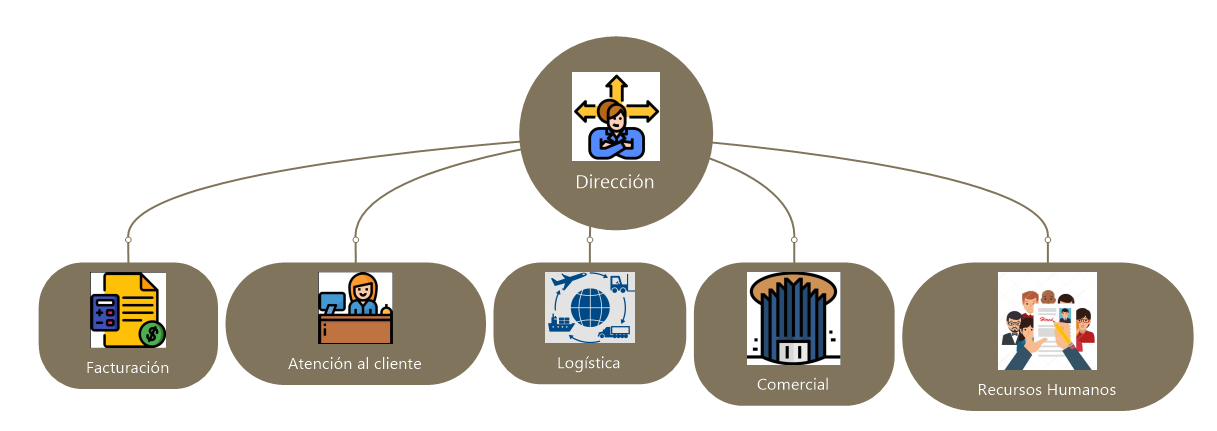
\includegraphics[scale=0.50]{imaxes/Organigrama.png}
	\caption{\label{fig:diagramaEstructura}Diagrama estructura - Formulario OM2}
\end{figure}

\section{Formulario OM-3: Descomposición del Proceso de Negocio.}

Descripción del proceso de interés a partir de las tareas que lo componen.

\begin{table}[H]
  \centering
  \resizebox{15,0cm}{!}{
    \begin{tabular}{|c|c|c|c|c|c|c|}
      \hline
      \multicolumn{3}{|c}{\textbf{Modelo de Organización}} & \multicolumn{4}{|c|}{\textbf{Formulario OM-3: Descomposición de los Procesos}}\\
      \hline \hline
      \textsc{N\textordmasculine} & \textsc{Tarea} & \textsc{Realiza\-da por} & \textsc{¿Dónde?} & \textsc{Recursos de Conocimiento} & \textsc {¿In\-ten\-si\-va en Conocimiento?} & \textsc{Im\-por\-tan\-cia} \\
      \hline

      1 & Recibimiento de los paquetes en la sucursal MRW (entrada) & \multicolumn{1}{|p{3.0cm}|}{\centering Repartidor experimentado} & \multicolumn{1}{|p{3.0cm}|}{\centering En la nave de la sucursal de MRW} & \multicolumn{1}{|p{5.0cm}|}{\centering No } & No & Requisito necesario para iniciar el proceso \\
      \hline
      2 & Generar lista de entregas según ruta asignada & \multicolumn{1}{|p{3.0cm}|}{\centering Repartidor experimentado} & \multicolumn{1}{|p{3.0cm}|}{\centering En la nave de la sucursal de MRW} & \multicolumn{1}{|p{5.0cm}|}{\centering Experiencia en reparto de paquetes según la ruta asignada} & Sí (bajo) & Máxima \\
      \hline
      3 & Determinar los recursos disponibles por la sucursal MRW para entregar según ruta & \multicolumn{1}{|p{3.0cm}|}{\centering Equipo Directivo, Repartidor experimentado} & \multicolumn{1}{|p{3.0cm}|}{\centering En la nave de la sucursal de MRW} & \multicolumn{1}{|p{5.0cm}|}{\centering Experiencia en distribución de recursos. Utilizar teoria de programación dinámica} & Sí (elevado) & Máxima \\
      \hline
      4 & Revisión y validación de la distribución de la paquetería & \multicolumn{1}{|p{3.0cm}|}{\centering Equipo Directivo} & \multicolumn{1}{|p{3.0cm}|}{\centering En la nave de la sucursal de MRW} & \multicolumn{1}{|p{5.0cm}|}{\centering Experiencia en distribución de recursos. Utilizar teoria de programación dinámica} & Moderado & Recomendable \\
      \hline      
    \end{tabular}
  }
	\caption{\label{tab:OM3}Descomposición del proceso de negocio - OM3}
\end{table}

\newpage
\section{Formulario OM-4: Activos de Conocimiento}
%%%%%%%%%%%%%%%%%%%%%%%%%%%%%%%%%%%%%%%%%%%%%%%%%%%%%%%%%%%%%%%%%%%%%%%%%%%%%%%

Descripción del componente \textit{conocimiento} del modelo de la organización.

\begin{table}[H]
  \centering
  \resizebox{15,0cm}{!}{
    \begin{tabular}{|c|c|c|c|c|c|c|}
      \hline
      \multicolumn{3}{|c}{\textbf{Modelo de Organización}} & \multicolumn{4}{|c|}{\textbf{Formulario OM-4: Activos de Conocimiento}}\\
      \hline \hline
      \textsc{Recurso de Conocimiento} & \textsc{Pertenece} & \textsc{Usado en} & \textsc{¿Forma Cor\-recta?} & \textsc{¿Lugar Cor\-recto?} & \textsc {¿Tiempo Cor\-recto?} & \textsc{¿Calidad Cor\-recta?} \\
      \hline
      
      \multicolumn{1}{|p{4.0cm}|}{\centering Experiencia en reparto de paquetes según la ruta asignada} & \multicolumn{1}{|p{3.0cm}|}{\centering Expertos en reparto} & \multicolumn{1}{|p{3.0cm}|}{\centering Tarea 2 de OM-3} & \multicolumn{1}{|p{3.0cm}|}{\centering Si, el conocimiento se puede adquirir con sistema de ubicación por código postal.} & Departamento de logística & - & \multicolumn{1}{|p{3.0cm}|}{\centering No} \\      
      \hline
      \multicolumn{1}{|p{4.0cm}|}{\centering Utilizar teoría de programación dinámica} & \multicolumn{1}{|p{3.0cm}|}{\centering Experto (director) y equipo directivo} & \multicolumn{1}{|p{3.0cm}|}{\centering Tarea 3 y 4 de OM-3} & \multicolumn{1}{|p{3.0cm}|}{\centering Sí, la teoría de programación dinámica proporciona unos estándares adecuados.} & Departamento de logística & - & \multicolumn{1}{|p{3.0cm}|}{\centering Sí} \\      
      \hline
      \multicolumn{1}{|p{4.0cm}|}{\centering Experiencia en distribución de recursos} & \multicolumn{1}{|p{3.0cm}|}{\centering Experto (director) y equipo directivo} & \multicolumn{1}{|p{3.0cm}|}{\centering Tarea 3 y 4 de OM-3} & \multicolumn{1}{|p{3.0cm}|}{\centering No} & Departamento de logística & - & \multicolumn{1}{|p{3.0cm}|}{\centering No}
      \\
      \hline
    \end{tabular}
  }
	\caption{\label{tab:OM4}Activos de conocimiento - OM4}
\end{table}


\section{Formulario OM-5: Análisis de viabilidad}


Elementos a considerar en el análisis de la viabilidad del proyecto. Nota: para mayor comodidad, en este apartado se puede prescindir del formato ``tabla'' y transformarla en subsecciones (comando subsubsection) manteniendo los mismos epígrafes de la primera columna.

\begin{table}[H]
  \centering
  \resizebox{15.0cm}{!}{
    \begin{tabular}{|l|l|} 
      \hline
      \textbf{Modelo de Organización} & \textbf{Formulario OM-5: Elementos del Documento de Viabilidad}\\ 
      \hline
      \hline

      \textsc{Viabilidad Empresarial} & \multicolumn{1}{p{14.0cm}|}{
      Al sustituir el trabajo de obra manual por un sistema automatizado; aumenta significativamente la velocidad en la tarea de asignación, lo cual supone también una reducción del coste, concretamente se reduce un 40\% el coste de mano de obra a principio de la jornada, además, al tener un sistema más preciso se evitan confusiones en la asignación.\newline
      Para llevar a cabo la implantación del sistema inteligente, la sucursal necesitará hacer una gran inversión: 
      \begin{itemize}
        \item Dos analistas durante cinco días (una semana) en una jornada completa (8 horas). Costo de $7.5 €/h$ con un total estimado de $600.00€$
        \item Cuatro desarrolladores trabajando diez días laborables (dos semanas) a jornada completa (8 horas). Costo de $7.5 €/h$ con un total estimado de $2400.00€$
        \item Un tester trabajando trabajando diez días (dos semanas) laborables a jornada completa (8 horas). Costo de $7.5 €/h$ con un total estimado de $600.00€$
        \item Dos técnicos trabajando cinco días laborables (una semana) a jornada completa (8 horas).Costo de $7.5 €/h$ con un total estimado de $600.00€$
        \item Empresa subcontratada para realizar la instalación de una cinta transportadora que garantiza la realización del trabajo en dos semanas.Costo total estimado de $10000.00€$ con todo el material incluido.
      \end{itemize}
      
      El proyecto no cambiaría el organigrama de la empresa ya que la parte que se hacía de forma manual ahora se hará de forma más automática, sin la necesidad de añadir/excluir algún departamento.

      Es un proyecto de riesgo bajo para el capital inicial invertido en ese proyecto, puesto que no afectará el funcionamiento de la empresa, ya que la misma ya se encuentra operativa y recibiendo beneficios de su operativa diaria.}\\
      \hline
    \end{tabular}
  }
  \caption{\label{tab:OM5}Formulario OM-5 (Parte 1). Viabilidad Empresarial}
\end{table}

\begin{table}[H]
  \centering
  \resizebox{15.0cm}{!}{
    \begin{tabular}{|l|l|} 
      \hline
      \textbf{Modelo de Organización} & \textbf{Formulario OM-5: Elementos del Documento de Viabilidad}\\ 
      \hline
      \hline

      \textsc{Viabilidad Técnica} & \multicolumn{1}{p{14.0cm}|}{
      La tarea a realizar tiene una baja complejidad técnica en el aspecto de conocimiento pues los problemas que se resolverán tienen una baja carga computacional para el sistema.\newline
      No hay impedimentos críticos de recursos o de tiempo, pues la empresa ya tiene su propia metodología en funcionamiento y suficientes ingresos como para evaluar la elaboración del proyecto con todos los recursos necesarios. \newline
      El éxito del proyecto estará determinado por la mejora en la calidad del servicio, la eficiencia de las entregas y en la satisfacción de todos los agentes involucrados en el mismo con la solución proporcionada. \newline
      La interacción con los usuarios finales del sistema (empleados de MRW) será sencilla y sin complejidad, prácticamente llevarán a cabo sus tareas rutinarias excepto las automatizadas por el sistema, además, los últimos (y futuros) avances en materia de accesibilidad a la tecnología y facilidad de uso, permitirán una usabilidad muy sencilla con nuestro sistema. \newline
      La interacción de este sistema con otros no sería complejo debido a que maneja fuentes de datos fácilmente parseables y flexibles (sistema de gestión de bases de datos que almacena datos de paquetes, flota, empleados y rutas). \newline
      El sistema no supodría un riesgo asociado a hipotéticos cambios tecnológicos en el futuro así como también posibles cambios en la legislación vigente sobre la protección datos.
      } \\
      \hline
    \end{tabular}
  }
  \caption{\label{tab:OM5-2}Formulario OM-5 (Parte 2). Viabilidad Técnica}
\end{table}

\begin{table}[H]
  \centering
  \resizebox{15.0cm}{!}{
    \begin{tabular}{|l|l|} 
      \hline
      \textbf{Modelo de Organización} & \textbf{Formulario OM-5: Elementos del Documento de Viabilidad} \\ 
      \hline
      \hline

      \textsc{Viabilidad del Proyecto} & \multicolumn{1}{p{14.0cm}|}{
        Con probabilidad hay un interés más que suficiente en la elaboración del proyecto debido a que podrá abaratar en gran medida los costes del proceso logístico de la empresa. \newline
        Los recursos están disponibles con facilidad debido a que la empresa ya está haciendo uso de la mayor parte de ellos y ya dispone de lo necesario.\newline
        El conocimiento y competencias necesarios ya están disponibles en los empleados de la empresa que ya están en su puesto. Implantar nuestra solución no requeriría ningún tipo de formación hacia los usuarios finales. \newline
        Las expectativas y resultados estimados de nuestro proyecto son realistas, pues al ser un proyecto con una baja complejidad hay holgura para posteriores cambios\dots

      } \\
      \hline
    \end{tabular}
  }
  \caption{\label{tab:OM5-3}Formulario OM-5 (Parte 3). Viabilidad del Proyecto}
\end{table}

\begin{table}[H]
  \centering
  \resizebox{15.0cm}{!}{
    \begin{tabular}{|l|l|} 
      \hline
      \textbf{Modelo de Organización} & \textbf{Formulario OM-5: Elementos del Documento de Viabilidad}\\ 
      \hline
      \hline
      
      \textsc{Acciones propuestas} & \multicolumn{1}{p{14.0cm}|}{Después del análisis realizado, se ha concluido que se llevará el proyecto adelante, incluyendo éste todas las tareas especificadas en el OM-3.\newline
      Instala un sistema de transporte de paquetes para agilizar y facilitar la logística.\newline
      Las acciones requeridas serian diseñar un motor de inferencia para sustituir al usuario experto para que tome decisiones de forma totalmente autónoma con una mínima entrada de datos que serían el riesgo que estamos dispuestos a asumir y el número máximo de operativas simultáneas a realizar.\newline
      Los riesgos serían tan sólo no lograr el funcionamiento adecuado del sistema, ya que en caso de fallos, la empresa podría seguir trabajando como lo hacía habitualmente sin problemas.} \\
      \hline
    \end{tabular}
  }
  \caption{\label{tab:OM5-4}Formulario OM-5 (Parte 4). Acciones Propuestas}
\end{table}
\clearpage